\documentclass[aspectratio=169,dvipsnames]{beamer}
\usepackage[utf8]{inputenc}
\usepackage[T1]{fontenc}
\usepackage{subfig}
\usepackage{amsmath}
\usepackage{mathtools}
\usepackage{booktabs}

\DeclareMathOperator*{\argmin}{arg\,min}



%%%%%%%%%%%%%%%%%%
% CHANGE command %
%%%%%%%%%%%%%%%%%%
\newcommand{\change}[0]{\color{blue}} % show blue
%\newcommand{\change}[0]{} % hide blue




\title{Don't Let Me Down!\\Offloading Robot VFs \\Up to the Cloud\vspace{1em}}

\date{June 20, 2023}
\author{K. Gillani (UC3M)\\
\textbf{J. Martín-Pérez} (UPM)\\
M. Groshev (UC3M)\\
A. de la Oliva (UC3M)\\
R. Gazda (ID)}

\usetheme{upm}

\begin{document}

\begin{frame}
\titlepage
\end{frame}

\begin{frame}{Overview}
    \tableofcontents
\end{frame}

\setcounter{framenumber}{0}


\section{Introduction}
\begin{frame}{\secname}
    Networked robotics interact with servers for, e.g.:
    \begin{itemize}
        \item remote driving; or
        \item assembly robots.
    \end{itemize}

    \vfill

    A remote driving Service $S$ has VFs:
    \begin{itemize}
        \item the robot drivers $v_1$; and
        \item the remote controller $v_2$.
    \end{itemize}
\end{frame}



\begin{frame}{\secname}
    The literature tends to offload -- e.g.
    the remote control $v_2$ -- to Edge, not to Cloud.

    \pause
    \vfill

    \emph{But channel impairments are still there!}

    Communication between VFs $(v_1,v_2)$ is harnessed.
\end{frame}


\subsection{Don't Let Me Down!}
\begin{frame}{\secname: \subsecname}
    \begin{figure}[t]%
        \subfloat[\label{fig:algosc} ]{{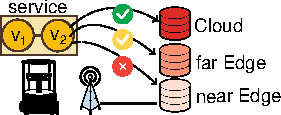
\includegraphics[width=0.35\columnwidth]{img/dlmd.pdf} }}\hfill
        \onslide<2->\subfloat[\label{fig:avoid} ]{{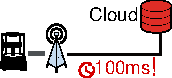
\includegraphics[width=0.24\columnwidth]{img/large-delay.pdf} }}\hfill
        \onslide<3->\subfloat[\label{fig:avoid-coverage} ]{{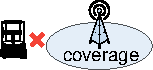
\includegraphics[width=0.24\columnwidth]{img/out-coverage.pdf} }}
    
        \caption{Don't Let Me Down! fosters
        offloading the robot service VFs up to
        the cloud (a), yet preventing the cloud
        large latencies (b)
        and running out of coverage (c).}
        \label{fig:dlmd}%
    \end{figure}
\end{frame}

%% \begin{frame}{\secname: \subsecname}
%%     Don't Let Me Down! \emph{optimizes} costs:
%%     \begin{itemize}
%%         \item taking offloading/migration decisions;
%%         \item handover decisions; and
%%         \item traffic steering decisions.
%%     \end{itemize}
%%     
%%     \vfill
%% 
%%     Don't Let Me Down! accounts for
%%     \begin{itemize}
%%         \item robot mobility;
%%         \item channel SNR; and
%%         \item classic capacity constraints.
%%     \end{itemize}
%% \end{frame}



\section{Problem Statement}


\subsection{Graph-based formulation}
\begin{frame}{\secname: \subsecname}
    Hardware graph $G$ with:
    \begin{itemize}
        \item robots $r\in V(G)$;
        \item radio PoA $R\in V(G)$;
        \item switches/routers $w \in V(G)$; and
        \item server nodes $n \in V(G)$
    \end{itemize}
    links are edges:
    \begin{itemize}
        \item wireless links $(r,R)\in E(G)$; and
        \item wired links $(n_1,n_2)\in E(G)$.
    \end{itemize}
\end{frame}


\begin{frame}{\secname: \subsecname}
    Robotic service graph $S$:
    \begin{itemize}
        \item VFs $v\in V(S)$; and
        \item VLs $(v_1,v_2)\in V(S)$.
    \end{itemize}
    The service $S$ asks for
    \begin{itemize}
        \item a maximum delay $D(S)$;
        \item computational resources $C(v),\ \forall v\in S$; and
        \item bandwidth resources $\lambda(v_1,v_2),\ \forall (v_1,v_2)\in E(S)$.
    \end{itemize}
\end{frame}


\subsection{Classic Decisions $a(n), a(n_1,n_2)$} 
\begin{frame}{\secname: \subsecname}
    The decisions to take are
    \begin{itemize}
        \item assigning VFs to servers $a(n)\subset S$; and
        \item assigning VLs to links $a(n_1,n_2)\subset E(S)$.
    \end{itemize}
    to minimize the deployment cost
    \begin{equation}
        \min_{a(n)} \sum_{n\in V(G)} \kappa_n |a(n)|
    \end{equation}
    with $\kappa_n\in\mathbb{R}^+$
    the server $n$ monetary cost, typically satisfying
    \begin{equation}
        \kappa_{\text{Cloud}} < \kappa_{\text{Edge}}
    \end{equation}
\end{frame}



\subsection{Wireless Decision $a(r,R)$}
\begin{frame}{\secname: \subsecname}
    Decide adequate PoA association/handovers
    $a(r,R)\in E(S)$ as the robot moves.
    \begin{equation}
        \sum_{\mathclap{(v_1,v_2)\in a(r_i,R_i)}} \lambda(v_1,v_2) \leq \mathrm{T}(r_i, R_i), \quad \forall (v_1,v_2)\in a(r_i,R_i)
        \label{eq:wireless-bandwidth-capacity}
    \end{equation}
    so wireless capacity is enough
    \begin{equation}
        \mathrm{T}(r_i,R_i) = (1-\delta(r_i,R_i))\lambda(r_i,R_i)\log_2\left(1+\frac{ \sigma_{R_i}(r_i)}{N}\right)
        \label{eq:channel-capacity}
    \end{equation}
    with $\delta(r_i,R_i)$ the PER and
    $\sigma_{R_i}(r_i)$ the signal strength.
\end{frame}



\section{Don't Let Me Down!}
\begin{frame}{\secname}
    A shortest-path based algorithm whose core idea is
    \begin{center}
        \emph{Don't Let the VFs go Down to the Edge!}
    \end{center}
    \vfill
    
    \begin{figure}[t]%
        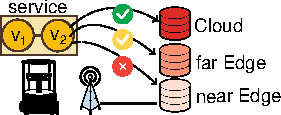
\includegraphics[width=0.35\columnwidth]{img/dlmd.pdf}
        \caption{Don't Let Me Down! sends VFs Up to the Cloud.}
    \end{figure}
\end{frame}

\subsection{the $\tau$ Metric}
\begin{frame}{\secname: \subsecname}
    Don't Let Me Down! is based on the $\tau$ metric
    \begin{align}
        \tau:\quad & \mathcal{P}\left( V(G)\right) \!\!\!\!\!\!\!\!\!\!\!\!\!\!\!\!\!\!\!\!\!\!\!\!\! &\longrightarrow & \quad  \mathbb{R}^+\\
                   & \qquad \mathcal{P}_0  \!\!\!\!\!\!\!\!\!\!\!\!\!\!\!\!\!\!\!\!\!\!\!\!\!\!\!\!\!\!\!\!\!\!\!\!\!\!\!&\longmapsto & \quad {\color{Red}\kappa_{\mathcal{P}_0[-1]}}
        + \sum_{(n_1,n_2)\in\mathcal{P}_0}
        \left(
            {\color{Green}\frac{1}{\lambda(n_1,n_2)}}
            + {\color{YellowOrange} d(n_1,n_2)}
        \right)
    \end{align}
    that fosters the use of
    \begin{itemize}
        \item {\color{Red} cheap servers} as the Cloud;
        \item {\color{Green} non-congested links}; and
        \item {\color{YellowOrange} fast links}.
    \end{itemize}
\end{frame}


\subsection{the Algorithm}
\begin{frame}{\secname: \subsecname}
    Don't Let Me Down! is summarized in three steps:
    \begin{enumerate}
        \item \emph{prune PoAs} without enough capacity $R\notin\{\hat{R}_i\}$
            \begin{equation}
                \{\hat{R}_i\} = \{R_i: \lambda(v_1,v_2) \leq T(r_i, R_i)\}_i
            \end{equation}
        \item find server to \emph{offload VFs} using
            \begin{equation}
                \text{Dijkstra}({source=}r\text{, weight=}\tau)
            \end{equation}
        \item \emph{select PoA} with best free/delay ratio
            \begin{equation}
                \argmin_{\hat{R}_i} \left\{\tfrac{1}{\lambda(r_i,\hat{R}_i)}+d(r_i,\hat{R}_i) \right\}
            \end{equation}
    \end{enumerate}
\end{frame}


%%%%%%%%%%%%%%%%%%%%%%%%%%%%%%%%%%%%%%%
%%%%%%%%%%%delay table%%%%%%%%%%%%%%%%%
%%%%%%%%%%%%%%%%%%%%%%%%%%%%%%%%%%%%%%%
\newcommand{\delaytab}{% Just for this example
    \begin{tabular}{c l l l }
        \toprule
         {\bf PoA} & {\bf Cloud} & {\bf  fEdge} & {\bf\ nEdge} \\ 
        \midrule
        R\textsubscript{1}, R\textsubscript{3} & 9~ms & 4~ms & 3~ms\\
       R\textsubscript{2}, R\textsubscript{4} & 18~ms & 8~ms & 9~ms\\
       R\textsubscript{5}, R\textsubscript{6} & 27~ms & 12~ms & 9~ms\\
       \bottomrule
    \end{tabular}
}

\section{Experimental evaluation}
\subsection{Ware Housing Scenario}
\begin{frame}{\secname: \subsecname}
\begin{figure}
    % trim=left bottom right top, clip
    \centering
    \subfloat[\label{fig:corridor} ]{{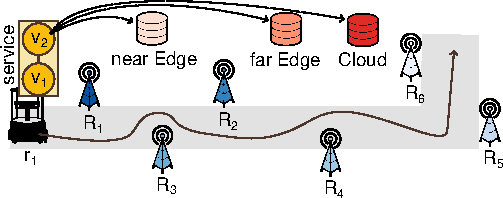
\includegraphics[width=0.4\columnwidth]{img/exp.pdf} }}
    
    \subfloat[\label{fig:oros} ]{{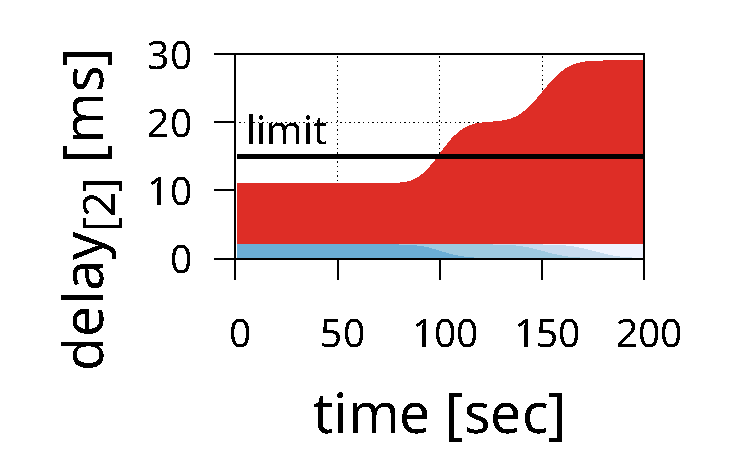
\includegraphics[trim=27 5 26 14,clip,width=0.25\columnwidth]{img/noDelay-stack.pdf} }}~
    \subfloat[\label{fig:tmc} ]{{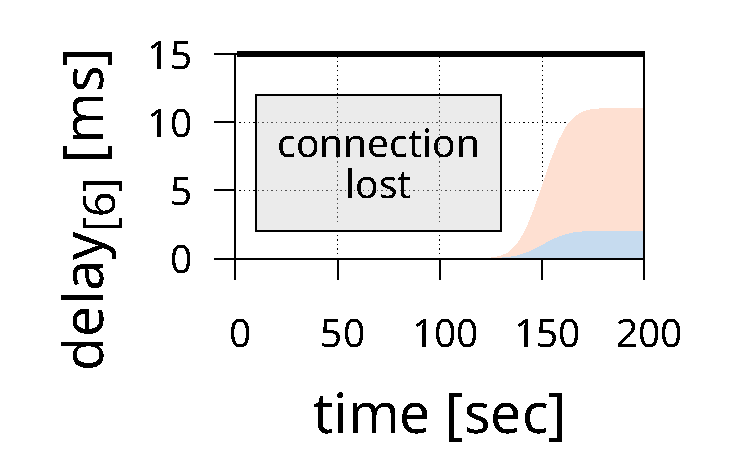
\includegraphics[trim=27 5 26 14,clip,width=0.25\columnwidth]{img/noT-stack.pdf} }}~
    \subfloat[\label{fig:dlmd-results} ]{{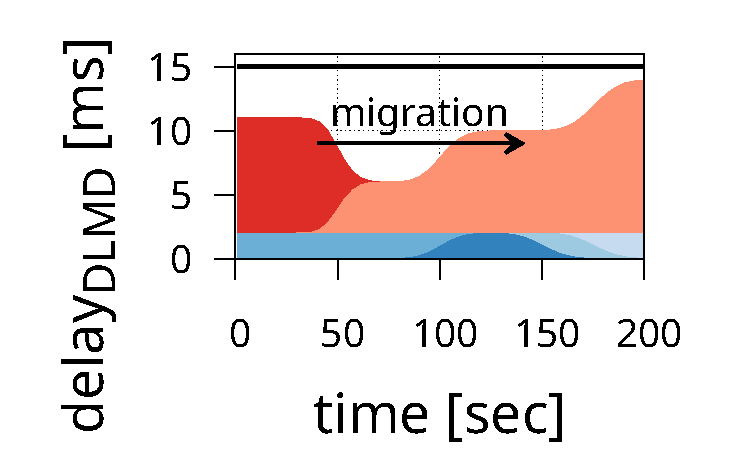
\includegraphics[trim=27 5 26 14,clip,width=0.25\columnwidth]{img/opt-stack.pdf} }}~
    
    \caption{Delay experienced by the robot
    using
    \cite{delgado2022oros},
\cite{delayandreliability} and Don't Let Me Down (DLMD).}
    \label{fig:exp-seup}
\end{figure}
\end{frame}




\subsection{Industrial scenario}
\begin{frame}{\secname: \subsecname}
\begin{figure}
    % trim=left bottom right top, clip
    \subfloat[\label{fig:pareto} ]{{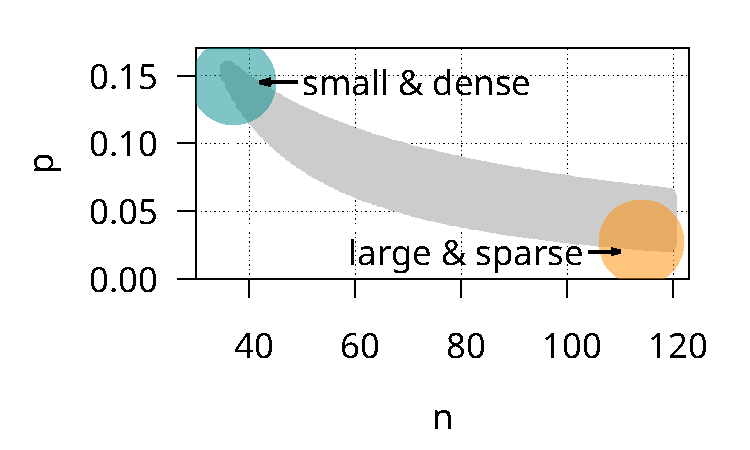
\includegraphics[trim=16 11 21 23,clip,width=0.4\columnwidth]{img/pareto-bound.pdf} }}~
    \subfloat[\label{fig:both-graphs} ]{{%
        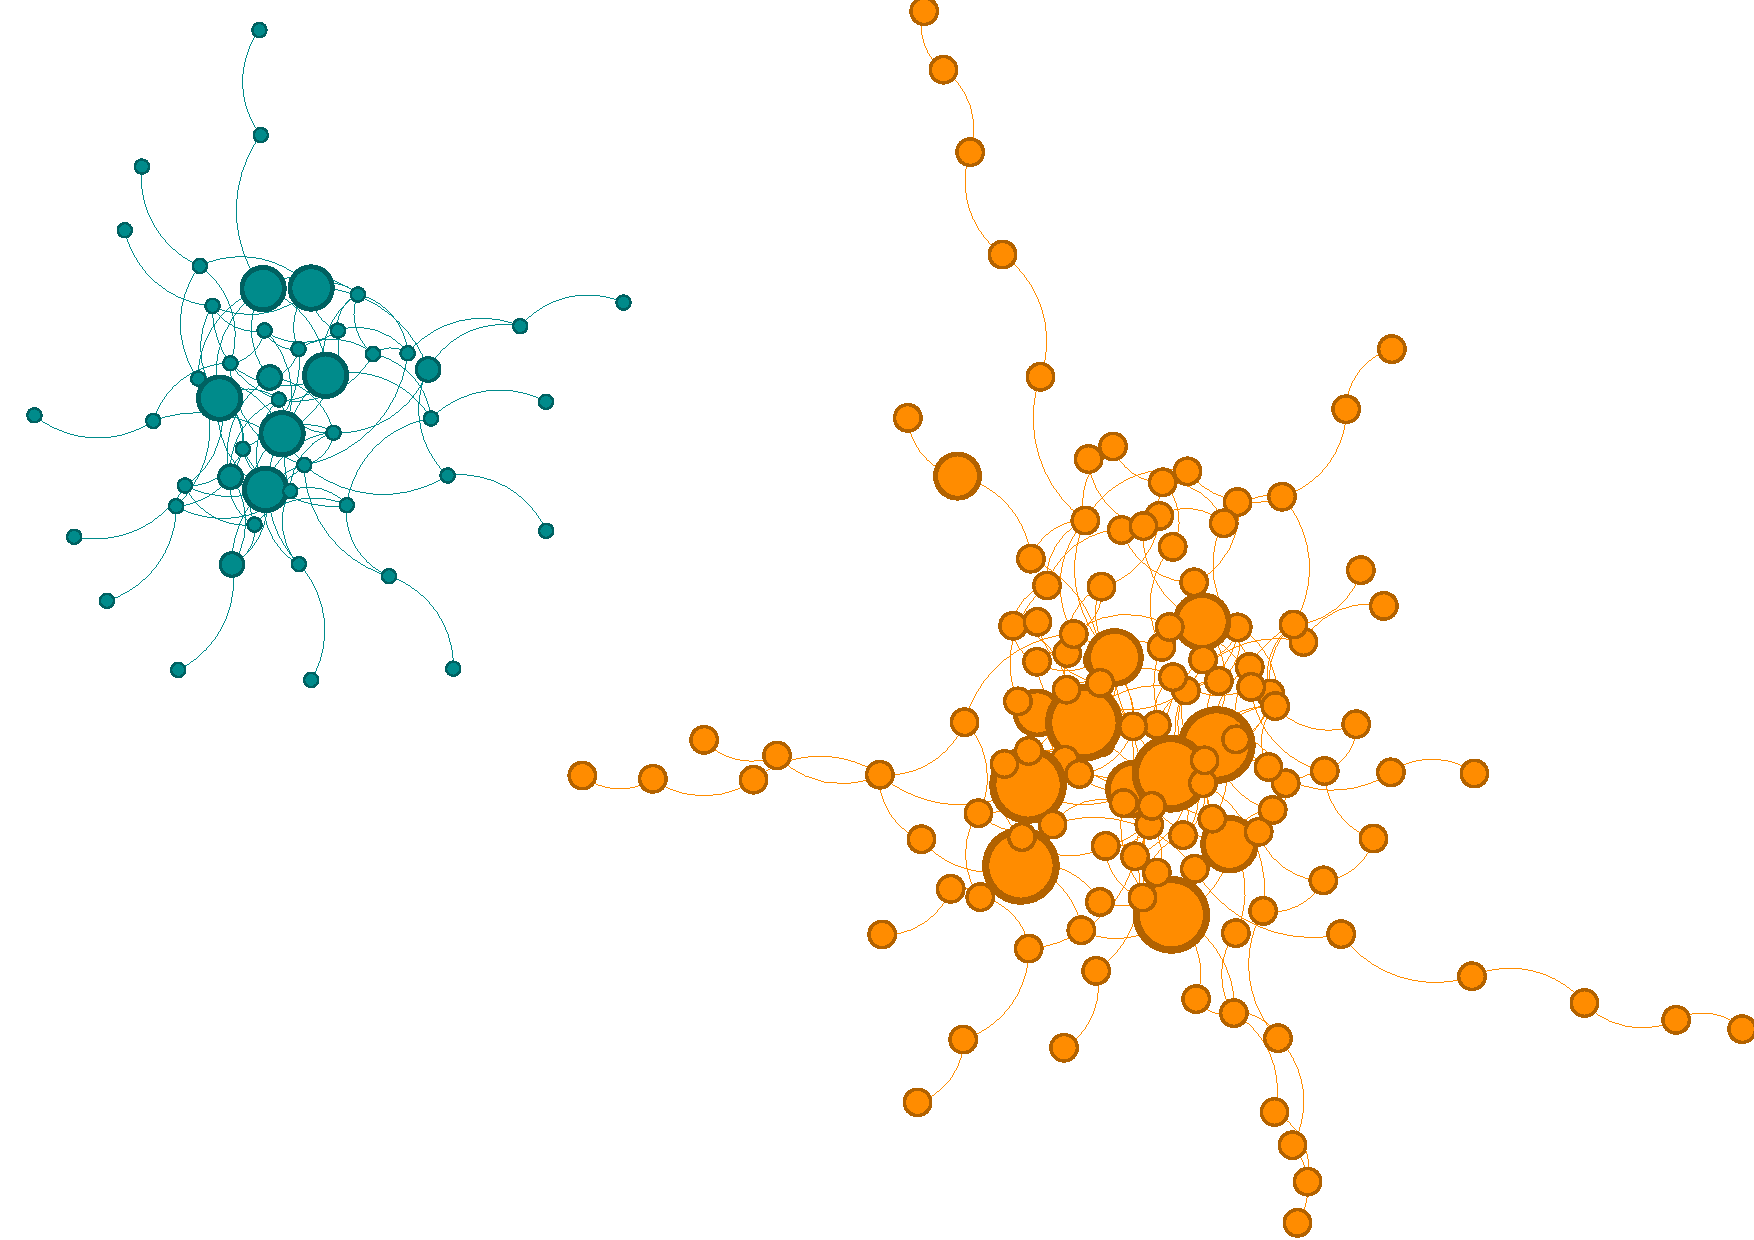
\includegraphics[width=0.3\columnwidth]{img/both_graphs.pdf} }}~
    \subfloat[\label{fig:urtinsa} ]{{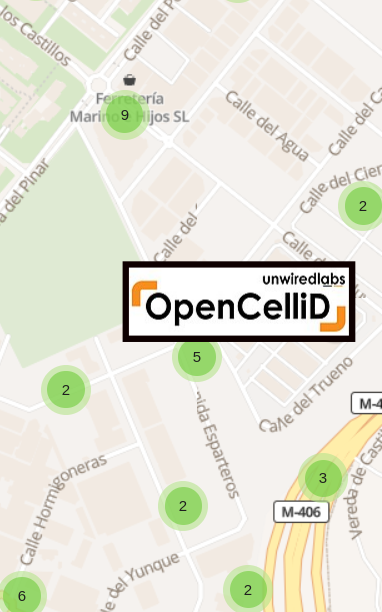
\includegraphics[width=0.17\columnwidth]{img/urtinsa-opencellid} }}
    
    \caption{Erdős–Rényi setups
    (a) network graphs (b) with PoAs of an
    industrial area (c).}
    \label{fig:industrial-setup}
\end{figure}
    
\end{frame}





\subsection{Industrial scenario II}
\begin{frame}{\secname: \subsecname}
\begin{figure}
    % trim=left bottom right top, clip
    \centering
    \subfloat[\label{fig:stress-delay} ]{{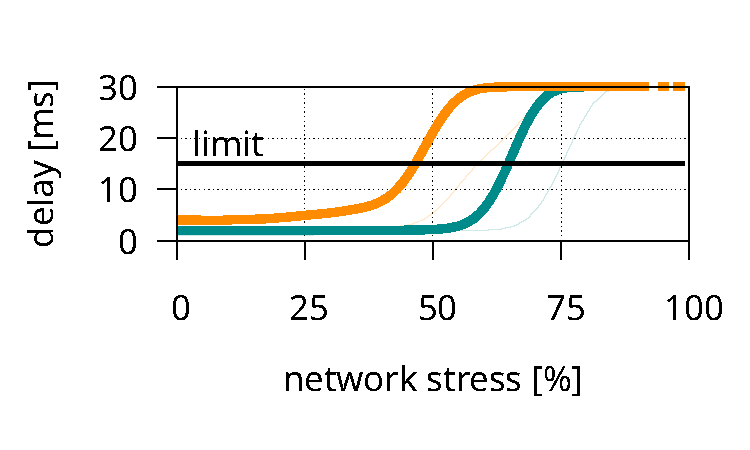
\includegraphics[trim=13 27 14 10, clip,width=.33\columnwidth]{img/stress-delay.pdf} }}~
    \subfloat[\label{fig:stress-edge} ]{{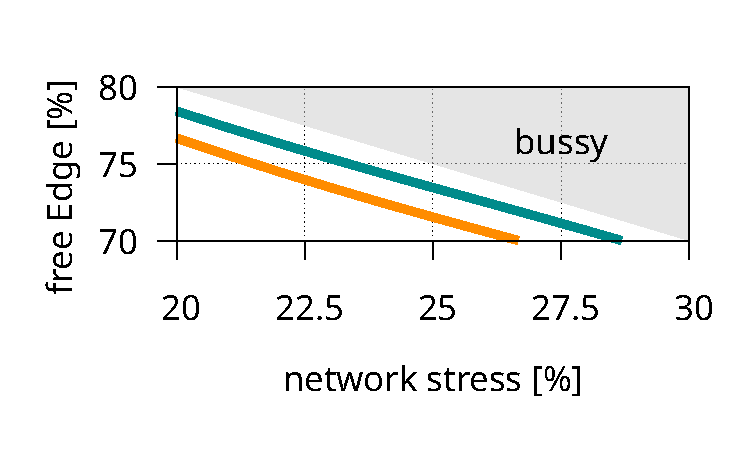
\includegraphics[trim=13 27 14 10, clip,width=.33\columnwidth]{img/stress-edge.pdf} }}\\[-.8em]
    \subfloat[\label{fig:stress-migrations} ]{{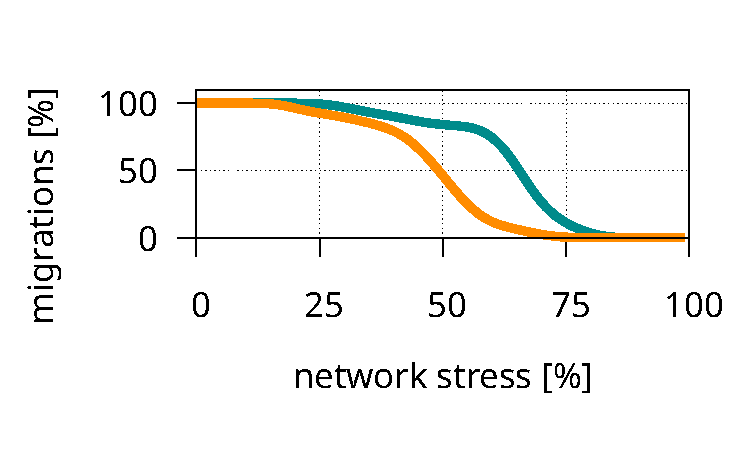
\includegraphics[trim=13 27 14 10, clip,width=.33\columnwidth]{img/stress-migrations.pdf} }}~
    \subfloat[\label{fig:stress-runtime} ]{{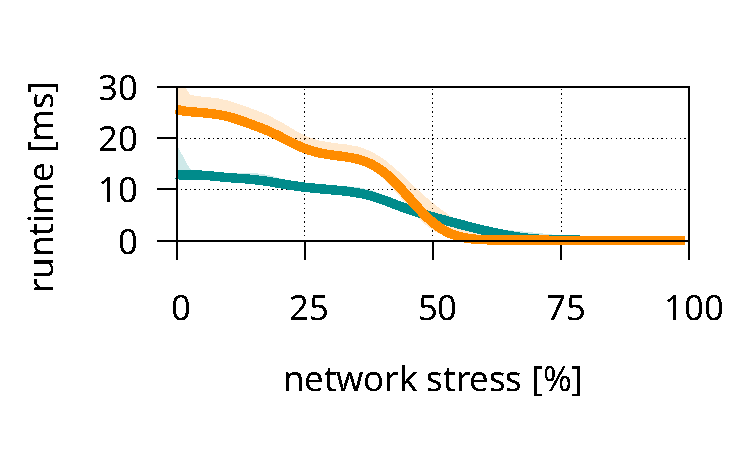
\includegraphics[trim=13 27 14 10, clip,width=.33\columnwidth]{img/stress-runtime.pdf} }}~
   \caption{DLMD stress test
    in Fig.~\ref{fig:industrial-setup}
    small (green) and large (orange)
    networks.}
   \label{fig:stress}%
\end{figure}
\end{frame}



\section{Conclusions \& Future Work}
\begin{frame}{\secname}
    Don't Let Me Down!
    \begin{itemize}
        \item takes $\sim 10$~[ms];
        \item reaches optimality in small scenarios (backup);
        \item offloads \& handovers to meet $<15$~[ms]; and
        \item minimizes Edge consumption.
    \end{itemize}

    \vfill

    Still to
    \begin{itemize}
        \item study w/ weighted $\tfrac{1}{\lambda}+d$
            metric for $\tau$;
        \item include SINR+propagation models; and
        \item study probabilistic mobility models.
    \end{itemize}
\end{frame}



\begin{frame}[allowframebreaks]
        \frametitle{Referencias}
        \bibliographystyle{ieeetr}
        \bibliography{refs.bib}
\end{frame}



\section*{Backup Slides}
\begin{frame}{\secname: \subsecname}
    \begin{figure}[t]
        % trim=left bottom right top, clip
        \centering
        \subfloat[\label{fig:compare-snr}   ]{{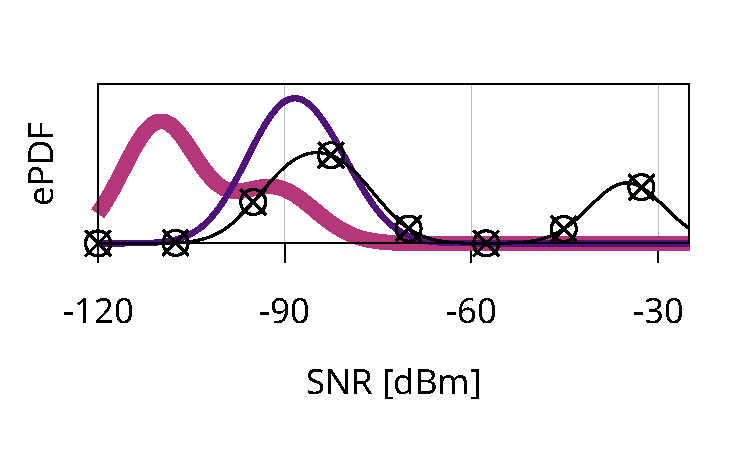
\includegraphics[trim=13 21 18 10, clip,width=.3\columnwidth]{img/snr-pdf.pdf} }}~
        \subfloat[\label{fig:compare-delay} ]{{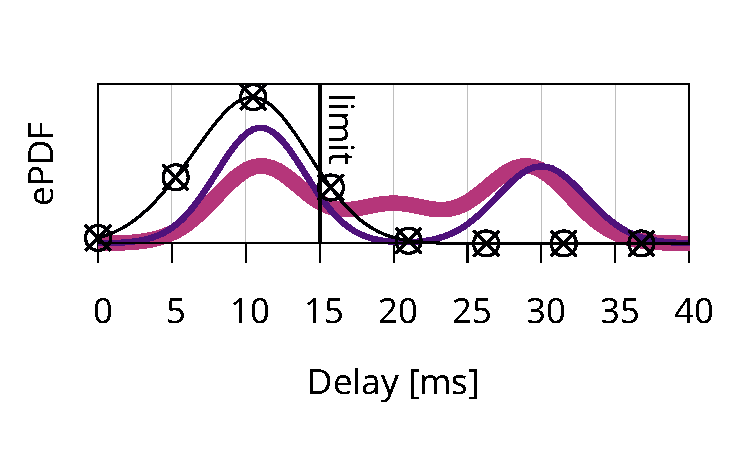
\includegraphics[trim=13 21 18 10, clip,width=.3\columnwidth]{img/delay-pdf.pdf} }}\\\vspace{-.7em}
        \subfloat[\label{fig:compare-cost}  ]{{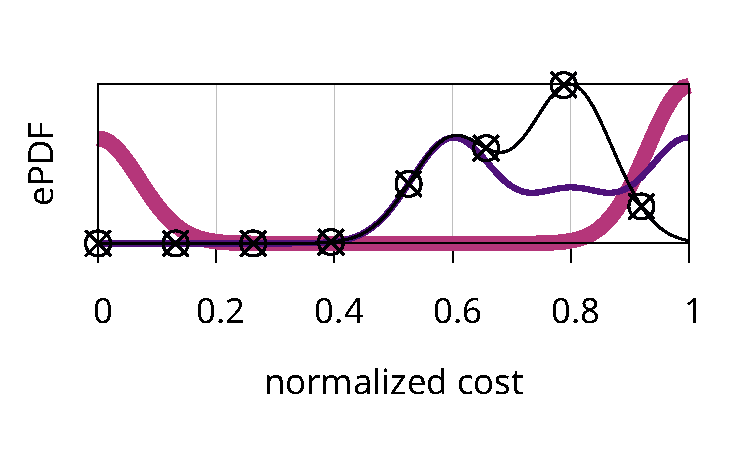
\includegraphics[trim=13 21 18 10, clip,width=.3\columnwidth]{img/cost-pdf.pdf} }}~
        \subfloat[\label{fig:compare-bw}    ]{{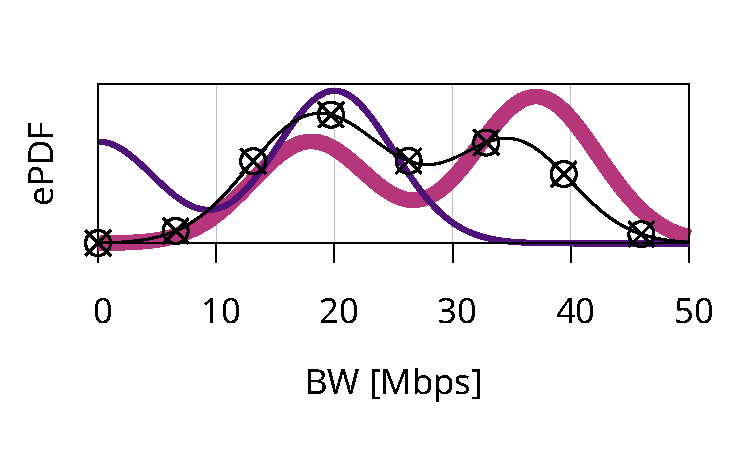
\includegraphics[trim=13 21 18 10, clip,width=.3\columnwidth]{img/bw-pdf.pdf} }}~
    
        
       \caption{Metrics' ePDFs
        using DLMD (circle),
        optimal (cross),
        \cite{delgado2022oros} (thickest), and
        \cite{delayandreliability} (thick)
       }%
       \label{fig:compare}%
    \end{figure}
\end{frame}




\end{document}
